\chapter{Timing attacks}
\index{Timing attacks}Come anticipato nel capitolo precedente, approfondiremo adesso la tipologia di attacchi basati sul tempo (timing attacks). 

I timing attacks si basano sulla misurazione del tempo necessario ad un dispositivo per effettuare un'operazione. Tali rivelazioni possono portare all'esposizione di alcune informazioni sull'operazione stessa o sui dati da essa manipolati. Questo accade perché molto spesso la durata di un'operazione dipende dagli input che vengono forniti dall'esterno.

Le istruzioni che prestano maggiormente il fianco a questo tipo di attacchi sono le istruzioni di branch e i condizionali.

\begin{center}
	\lstinputlisting[language={Java}, caption={esempio di funzione vulnerabile ad un timing attack}, label={list:timingBase}, frame={none},basicstyle={\small\ttfamily}]{code/timingBase.txt}
\end{center}

Ad esempio, un programma implementato con il \cref{list:timingBase}, se fatto girare con la stringa "\texttt{passwordToBeStolen}" impiegherà un tempo maggiore rispetto allo stesso programma fatto girare con la stringa "\texttt{foo}". Nel primo caso infatti verrà scansionata tutta la stringa, mentre nel secondo caso si interromperà immediatamente. Questa informazione può essere utilizzata dall'attaccante che, procedendo per tentativi, può arrivare a ricavare la stringa esatta.

Questo esempio banale non deve portare a pensare che le caratteristiche temporali di una certa operazione rivelino solamente informazioni su una piccola parte di un intero sistema crittografico. Come dimostrato da \emph{Kocher} in \cite{kocher1996timing} esistono attacchi che, solamente sfruttando misurazioni di tempi di esecuzione di particolari operazioni, riescono a scoprire l'intera chiave in implementazioni diverse di algoritmi crittografici complessi come \emph{RSA}, \ac{DH} o \ac{DSS}.

Per ottenere tali risultati, le misurazioni dei tempi vengono analizzate con un modello statistico che scopre la chiave con un certo intervallo di confidenza, progredendo di un bit alla volta. Il modello deve essere in grado di controllare la correlazione tra le varie misurazioni e stabilire di conseguenza se il successivo bit della chiave debba essere $0$ oppure $1$.

	\section{Attacchi reali}
	
	Analizziamo tre attacchi reali presi proprio dall'articolo di \emph{Kocher}.
	
		\subsection{Esponenziazione modulare}
		Un'operazione comune utilizzata sia da \ac{DH} che da RSA è il calcolo di $$R = y^{x} \ mod \ n.$$ In questa operazione, $n$ è pubblico e $y$ può essere trovato tramite una qualche intercettazione di messaggi da parte dell'attaccante. Lo scopo finale dell'attacco sarà quello di trovare $x$, la chiave segreta.
		
		Per questo attacco, fissata una $x$, la vittima deve calcolare $y^{x} \ mod \ n$ per diversi valori di $y$, e l'attaccante deve conoscere $y$, $n$ e il tempo necessario al calcolo.
		Analizzando statisticamente queste misurazioni, si riesce a risalire all'intera chiave segreta.
		
		Le informazioni necessarie e le misurazioni temporali posso essere ottenute passivamente tramite qualche forma di intercettazione (ad esempio creando un \emph{man-in-the-middle}) sul protocollo di comunicazione fornito dalla vittima. L'attaccante a questo punto conosce il messaggio ricevuto dalla vittima e misura il tempo che essa impiega per rispondere con il risultato utilizzando vari $y$.
		
		Questo attacco può essere adattato ad ogni implementazione di questa operazione, all'unica condizione che non si tratti di una delle varianti che lavora in tempo costante.
		
		\subsection{Moltiplicazione di Montgomery e Chinese Remainder Theorem}
		In un'operazione di moltiplicazione modulo $n$, il passo di riduzione modulare è il principale responsabile delle variazioni nel tempo di esecuzione. La moltiplicazione di \emph{Montgomery}\cite{montgomery1985modular} elimina il passo di riduzione modulo $n$ riducendo il tempo totale dell'operazione e, di conseguenza, anche le variazioni associate.
		
		Per ottimizzare le operazioni che utilizzano la chiave privata di RSA viene utilizzato anche il \ac{CRT}. Se il messaggio da cifrare è $y$, utilizzando il \ac{CRT} si calcolano inizialmente $(y \ mod \ p)$ e $(y \ mod \ q)$. Queste due operazioni iniziali sono la parte dell'algoritmo vulnerabile ai timing attacks. Il più semplice di questi attacchi sceglie un valore $y$ che si suppone vicino a $p$ o $q$. Successivamente utilizza i tempi di esecuzione per capire se $y$ sia più grande o più piccolo di $p$ (o di $q$). Se $y < p$, il calcolo di $y \ mod \ p$ non esegue alcuna operazione, mentre se $y \geq p$, sarà necessario sottrarre $p$ da $y$ almeno una volta aumentando il tempo di esecuzione.
		
		Le caratteristiche esatte dell'attacco dipendono dall'implementazione dell'algoritmo attaccato.
		
		\subsection{Digital Signature Algorithm}
		Il \ac{DSA} è uno standard \ac{FIPS} per la firma digitale proposto dal \ac{NIST} nell'agosto del 1991 per essere impiegato nel \ac{DSS}, e adottato definitivamente nel 1993. Le sue specifiche sono contenute nel documento \ac{FIPS}-186\cite{kravitz1993digital}.
		
		Il \ac{DSS} calcola $s = (k^{-1}(H(m) + x \cdot r)) \ mod \ q$ dove $r$ e $q$ sono noti all'attaccante, $k^{-1}$ è precalcolato, $H(m)$ è l'hash del messaggio e $x$ è la chiave privata.
		
		Se l'operazione di riduzione modulo $q$ non è stata implementata per funzionare a tempo costante, esiste una correlazione tra il tempo totale di computazione e quello necessario per eseguire $(x \cdot r \ mod \ q)$. L'attaccante può quindi calcolare tale tempo in modi simili a quelli visti in precedenza, e scoprire la chiave segreta $x$.
		
	\section{Generalizzazione}
	Abbiamo appena illustrato tre casi concreti di timing attacks contro specifici algoritmi crittografici. Partendo da queste basi, abbiamo cercato una generalizzazione applicabile alla maggior parte degli attacchi di questo tipo.
	
	Abbiamo notato che tutte le informazioni che vengono ricavate sono connesse alle variazioni del tempo di esecuzione, e dipendono in qualche modo dal segreto che l'attaccante vuole scoprire.
	
	Abbiamo supposto che l'attaccante prenda di mira una specifica istruzione \texttt{if} nel codice, come ad esempio \texttt{if p(h) then c} dove \texttt{p(.)} è un predicato con valore $0/1$ su \texttt{h}, in un contesto \texttt{B[.]}. In questo caso, l'intero programma sarebbe \texttt{B[if p(h) then c]}.
	
	Abbiamo assunto che il tempo di esecuzione dipenda da alcuni input forniti al programma che modificano l'esecuzione di \texttt{c}. Considerando i.i.d questi input e fissando il segreto \texttt{h}, abbiamo definito il tempo di esecuzione dell'intero programma come una variabile aleatoria $\tcal$ che può essere divisa in \begin{equation} \label{eq:1}
		\tcal = \talfa + \text{\texttt{p(h)}}\cdot \tbeta
	\end{equation} 
	dove $\talfa$ è il tempo di esecuzione dovuto a \texttt{B} e $\tbeta$ quello dovuto a \texttt{c} in una completa esecuzione di \texttt{B[c]}.
	
	Lo scopo dell'attaccante è quello di scoprire il valore di \texttt{p(h)} (che potrebbe rappresentare l'i-esimo bit della chiave) attraverso misurazioni del tempo di esecuzione dell'intero programma.
	
	A questo proposito è immediato vedere che $$var(\tcal)=\left\{\begin{array}{ll}
	var(\talfa) & \mathrm{s}\mathrm{e}\ \text{\texttt{p(h)}} = 0\\
	var(\talfa)+var(\tbeta)+2\cdot cov (\talfa,\tbeta) & \mathrm{s}\mathrm{e}\ \text{\texttt{p(h)}} = 1
	\end{array}\right.$$ 
	
	da cui ricaviamo che $$var(\tcal) > var(\talfa) \Leftrightarrow \text{\texttt{p(h)}} = 1$$ 
	
	a condizione che 
	\begin{equation} \label{eq:2}
		var(\tbeta) > 2 \cdot |cov(\talfa,\tbeta)|.
	\end{equation}
		
	Questa formulazione però non è sufficiente per l'attaccante visto che, sebbene possa stimare facilmente $var(\tcal)$, non ha modo di stimare $var(\talfa)$ a meno che non sia in grado di eseguire \texttt{B} in isolamento (ipotesi troppo forte e poco realistica). Abbiamo pensato che l'attaccante potrebbe però simulare \texttt{c}, calcolare $\tbeta$ e confrontare $var(\tcal - \tbeta)$ con $var(\tcal)$. 
	
	Il risultato che abbiamo ottenuto è stato dimostrare che $$var(\tcal - \tbeta) < var(\tcal) \Leftrightarrow \text{\texttt{p(h)} = 1}.$$ Questi sono tutti valori calcolabili (o perlomeno stimabili).\\
	
	\subsection{Dimostrazione} 
		Dimostrazione $\Leftarrow$:\\
		Se $\text{\texttt{p(h)}} = 1$, allora dall'\cref{eq:1} $$\tcal = \talfa + \tbeta \Rightarrow \tcal - \tbeta = \talfa$$
		da ciò si deduce che $$var(\tcal - \tbeta) = var(\talfa)$$ 
		e che $$var(\tcal) = var(\talfa) + var(\tbeta) + 2cov(\talfa,\tbeta)$$
		e quindi per l'\cref{eq:2} $$var(\tcal - \tbeta) < var(\tcal).$$\\Dimostrazione $\Rightarrow$:\\
		In questo caso dimostriamo la contronominale $$\text{\texttt{p(h)}} = 0 \Rightarrow var(\tcal - \tbeta) \geq var(\tcal).$$  
		Dall'\cref{eq:1} sappiamo che
		\begin{equation} \label{eq:3}
			\text{\texttt{p(h)}} = 0 \Rightarrow \tcal = \talfa + 0\cdot \tbeta = \talfa
		\end{equation}
		da cui si deduce che $$var(\tcal) = var(\talfa).$$
		Dall'\cref{eq:3} troviamo che
		$$\tcal = \talfa \Rightarrow \tcal - \tbeta = \talfa - \tbeta$$
		e quindi
		$$var(\tcal - \tbeta) = var(\talfa) + var(\tbeta) - 2\cdot cov (\talfa,\tbeta)$$
		da cui per l'\cref{eq:2}
		$$var(\tcal - \tbeta) > var(\talfa) = var(\tcal).$$
		\begin{flushright}
			$\square$
		\end{flushright}

	\subsection{Validazione sperimentale}
		La generalizzazione precedente, a causa della condizione richiesta nell'\cref{eq:2}, potrebbe apparire come un semplice esercizio di stile teorico con poche applicazioni pratiche. Per questo motivo abbiamo cercato di dimostrare sperimentalmente che tale condizione si verifica normalmente anche nella realtà.
		
		Abbiamo creato una implementazione dell'algoritmo di esponenziazione modulare (appendice A), una delle funzioni crittografiche maggiormente interessate dai timing attacks. Questo algoritmo calcola $$y = x^k \ mod \ n,$$ dove $x$ e $n$ sono interi positivi e $k$ è la chiave segreta, nel seguente modo: 
		
		\begin{center}
			\begin{lstlisting}[caption={algoritmo di esponenziazione modulare},label={list:espMod}]
			y = 1;
			per ogni bit i di k
				se k[i] == 1
					y = y * y
					y = y * x
					y = y mod n
				altrimenti
					y = y * y
					y = y mod n
			\end{lstlisting}
		\end{center}
	
		L'istruzione presa di mira dall'attacco è il controllo sull'i-esimo bit della chiave. Abbiamo instrumentato il codice in maniera tale da ottenere $\talfa \text{ e } \tbeta$ per poterne poi calcolare varianze e covarianze. Il programma esegue $1000$ volte l'intero algoritmo scegliendo casualmente $x\text{,}k\text{ e }n$. Per ogni esecuzione, il campionamento di $\talfa$ viene eseguito ad ogni iterazione, mentre quello di $\tbeta$ viene eseguito solamente nell'iterazione nella quale compare il primo '1' della chiave. In questo modo emuliamo il comportamento dell'attaccante che può simulare \texttt{c} in isolamento. Con questi $1000$ campioni si calcolano $var(\tbeta)$ e $covar(\talfa,\tbeta)$ e si effettua il controllo richiesto dall'\cref{eq:2}.
		
		Questa procedura viene ripetuta $100$ volte per ogni esperimento e, alla fine, viene restituito il numero di volte in cui l'equazione risulta soddisfatta.
		
		Per avere risultati più significativi, il tutto viene ripetuto per $10$ volte e viene restituita la media.
		
		\begin{figure}
			\begin{center}
				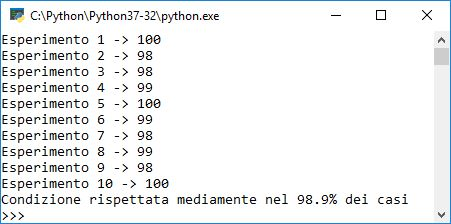
\includegraphics[width=.9\textwidth]{resPython}
				\caption{esecuzione del test di validazione}
				\label{fig:resPython}
			\end{center}
		\end{figure}
	
		Come si vede in \cref{fig:resPython}, in media, in più del $98\%$ delle esecuzioni l'equazione è effettivamente verificata.	Possiamo quindi affermare che la condizione imposta sia assolutamente plausibile. 	 		

	\section{Contromisure ai timing attacks}
	Illustriamo adesso alcune precauzioni che possono essere prese per difendersi dai timing attacks.
	
	\subsection*{Computazione indipendente da input o chiavi}
		La prima contromisura che può essere applicata è quella di rendere indipendente dagli input o dalla chiave il tempo d'esecuzione delle funzioni più critiche. Nel momento in cui una di queste funzioni dovesse aver bisogno di utilizzare tali dati, quella funzione deve essere implementata in modo tale da restituire un tempo di computazione costante (in termini di cicli di clock).
		
		Questa tecnica risolve completamente il problema dei timing attacks, ma diminuisce le prestazioni del programma. Questo è dovuto al fatto che alcune ottimizzazioni proposte nel tempo per velocizzare la computazione di tali funzioni dipendono da una particolare gestione degli input o della chiave, e quindi non possono essere applicate.
		
	\subsection*{Blinding}
		Un'altra contromisura, introdotta da \emph{Chaum} in \cite{chaum1983blind}, consiste nel "nascondere" l'utilizzo di input esterni e di chiavi, modificandoli in maniera opportuna. Ad ogni esecuzione, ad esempio, potrebbe essere aggiunta una quantità casuale alla chiave o all'esponente utilizzato nell'esponenziazione modulare che, modificandoli, renda sempre diverso il tempo di computazione.
		
		Nell'utilizzare questa tecnica è necessario prestare attenzione al fatto che le quantità aggiunte non presentino a loro volta delle regolarità statistiche che potrebbero essere analizzate dall'attaccante, rilevate e compensate.
		
	\subsection*{Rimozione delle istruzioni di branch}
		In \cite{schwabe2016counter}, \emph{Schwabe} propone di implementare funzioni sensibili senza utilizzare istruzioni di branch. Eliminare tali istruzioni permette infatti di uniformare i tempi di esecuzione rendendo molto più difficile l'attuazione dei timing attacks.
		
		Se ad esempio prendiamo il \cref{list:timing} ci accorgiamo che il programma ha tempi di esecuzione diversi in base al valore del segreto.
		
		\begin{center}
			\begin{lstlisting}[language={C},caption={codice da proteggere},label={list:timing}]
				if (secret) {
					r = doA(); /* long operation*/
				} else {
					r = doB(); /*short operation*/
				}
			\end{lstlisting}
		\end{center}
		
		Per osservare i risvolti pratici di questo problema, prendiamo un'implementazione di una delle operazioni più critiche di RSA: l'esponenziazione modulare (\cref{list:square1}).
		
		\begin{center}
			\begin{lstlisting}[language={C},caption={RSA, esponenziazione modulare v1},label={list:square1}]
				typedef unsigned long long uint64;
				typedef uint32_t uint32;
				uint32 modexp(uint32 a, uint32 mod, unsigned char exp[4]) {
					int i,j;
					uint32 r = 1;
					for(i=3;i>=0;i--) {
						for(j=7;j>=0;j--) {
							r = ((uint64)r*r) % mod;
							if(exp[i] & (1<<j))
								r = ((uint64)a*r) % mod;
						}
					}
					return r;
				}
			\end{lstlisting}
		\end{center}
		
		Le istruzioni a riga $9-10$ che eseguono una moltiplicazione ed una riduzione modulare solo se l'i-esimo bit dell'esponente è pari a $1$, sono quelle che potrebbero fornire le informazioni temporali all'attaccante.
		
		La prima modifica che può venire in mente per risolvere questo problema è di far eseguire le stesse operazioni ad entrambi i rami della branch, modificando la funzione come nel \cref{list:square2}. In questo modo, a prescindere dal risultato del controllo, verranno effettuate comunque una moltiplicazione ed una riduzione modulare, uniformando il tempo di esecuzione.
		
		\begin{center}
			\begin{lstlisting}[language={C},caption={RSA, esponenziazione modulare v2},label={list:square2}]
			typedef unsigned long long uint64;
			typedef uint32_t uint32;
			uint32 modexp(uint32 a, uint32 mod, unsigned char exp[4]) {
				int i,j;
				uint32 r = 1, t;
				for(i=3;i>=0;i--) {
					for(j=7;j>=0;j--) {
						r = ((uint64)r*r) % mod;
						if(exp[i] & (1<<j)){
							r = ((uint64)a*r) % mod;
						} else {
							t = ((uint64)a*r) % mod;
						}
					}
				}
				return r;
			}
			\end{lstlisting}
		\end{center}
	
		Questa soluzione è purtroppo inefficace perché qualunque compilatore si accorgerebbe del fatto che la variabile \texttt{t} non viene mai utilizzata, ottimizzando il codice con la rimozione di quell'istruzione. Se anche evitassimo tutte le ottimizzazioni da parte del compilatore (subendo una notevole perdita di prestazioni generali del programma), potremmo comunque non ottenere un tempo costante a causa di altre ottimizzazioni (inevitabili) a livello di processore, come ad esempio la \emph{branch prediction}.
		
		La soluzione proposta è quella di eliminare completamente l'istruzione di branch come nel \cref{list:square3}.
		
		\begin{center}
			\begin{lstlisting}[language={C},caption={RSA, esponenziazione modulare v3},label={list:square3}]
			uint32 modexp(uint32 a, uint32 mod, const unsigned char exp[4]) {
				int i,j;
				uint32 r = 1,t;
				for(i=3;i>=0;i--) {
					for(j=7;j>=0;j--) {
						r = ((uint64)r*r) % mod;
						t = ((uint64)a*r) % mod;
						cmov(&r, &t, (exp[i] >> j) & 1);
					}
				}
				return r;
			}
			\end{lstlisting}
		\end{center}
	
		In questa implementazione vengono sempre eseguite entrambe le operazioni (sia su \texttt{r} che su \texttt{t}) e si nota l'utilizzo dell'istruzione assembly \texttt{cmov} (\emph{conditional move}). Questa istruzione non fa uso di alcuna predizione sulla branch ed ha bisogno sia del valore di \texttt{r} che del valore \texttt{t}, che quindi non possono essere ottimizzati.
		